\documentclass[compress]{beamer}
\usetheme{hitszbeamer}
\usepackage{booktabs}
\usepackage{bm}

\begin{document}

\graphicspath{{figures/}}

\title[基于神经网络和树搜索的五子棋AI]{基于神经网络和树搜索的五子棋AI\\[2mm] 中期答辩}
\author[王梓尧]{答辩人:修泽\\[2mm] 组员:王梓尧 \hspace{2pt} 修泽}
\institute[哈尔滨工业大学]{\small  哈尔滨工业大学}
\date{\small \vskip -10pt 2023年2月12日}

\begin{frame}
  \maketitle
\end{frame}

\section*{目录}
\frame{
  \frametitle{\secname}
  \tableofcontents[hideallsubsections]
}

\section{研究内容}

\begin{frame}{研究内容}
  \begin{itemize}
	\item 五子棋对局的实现
    \item 蒙特卡洛树搜索
    \item 神经网络
  \end{itemize}
\end{frame}

\subsection{五子棋对局}
\begin{frame}{后端架构}
  \begin{itemize}
	\item 定义 Board 类,记录棋盘数据。支持查询棋盘坐标的状态,落子,以及清空棋盘。 
		\pause
	\\[5mm]
    \item 定义 Player 类,给出棋手对棋盘的操作的方法
    \item 分别实现 GomokuAI 和 Person 两个子类,分别实现 AI 与人类玩家的操作。
		\pause
	\\[5mm]
    \item 定义 Rule 类,完成对棋盘坐标是否可以落子,及是否终局的判断。
	\item 同时完成落子到棋盘上操作
  \end{itemize}
\end{frame}

\begin{frame}{前端实现}
  \begin{itemize}
    \item 使用 TKinter 模块的 canvas 组件完成棋盘的绘制
    \item 同时可完成对鼠标操作的绑定
		  \pause
	\\[5mm]
	\item 使用 TKinter 模块的 botton 组件完成相应按钮的创建
  \end{itemize}
\end{frame}

\begin{frame}{前端展示}
  \begin{figure}[htbp]
    \centering
    \begin{minipage}[t]{0.4\textwidth}
      \centering
      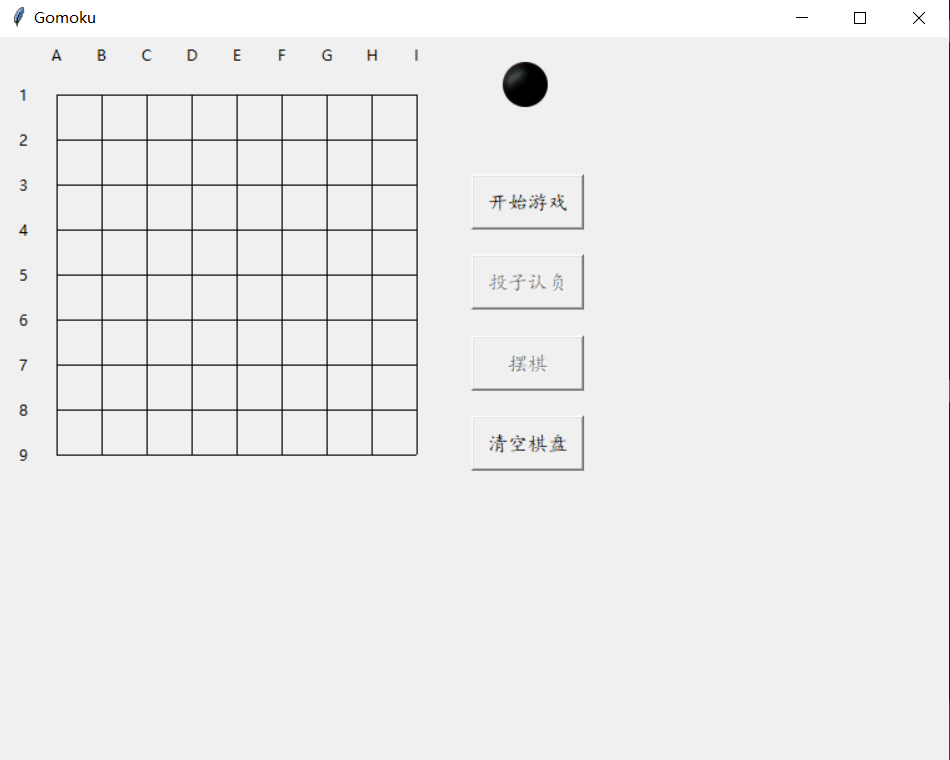
\includegraphics[width=3cm]{uiempty.png}
    \end{minipage}
    \begin{minipage}[t]{0.4\textwidth}
      \centering
      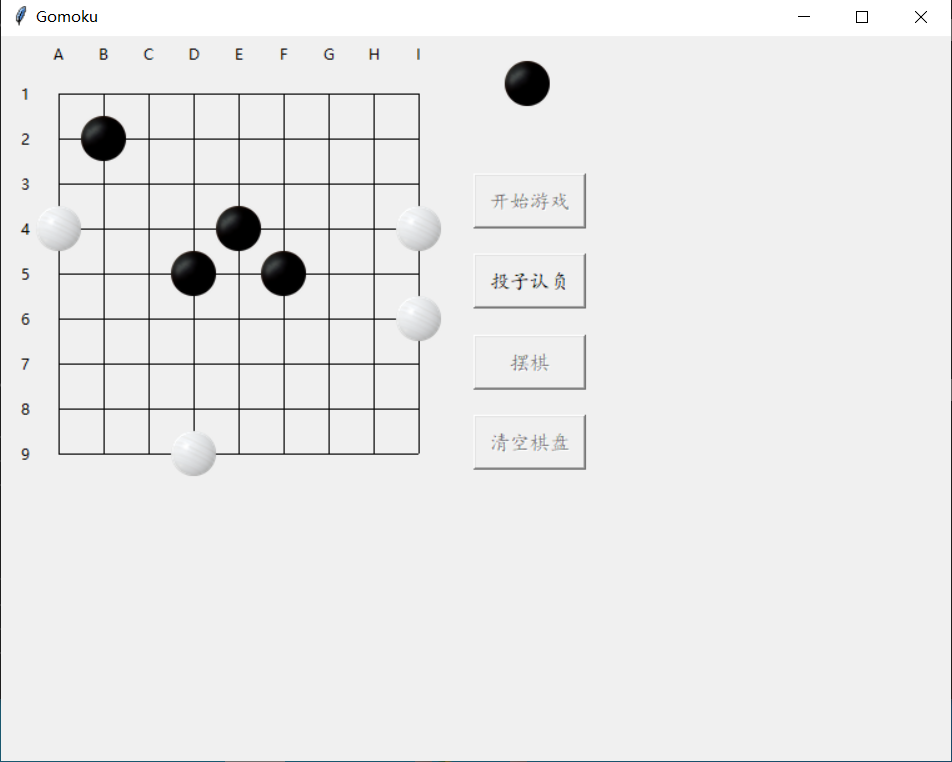
\includegraphics[width=3cm]{uihalf.png}
    \end{minipage}
	\\[5mm]
    \begin{minipage}[t]{0.4\textwidth}
      \centering
      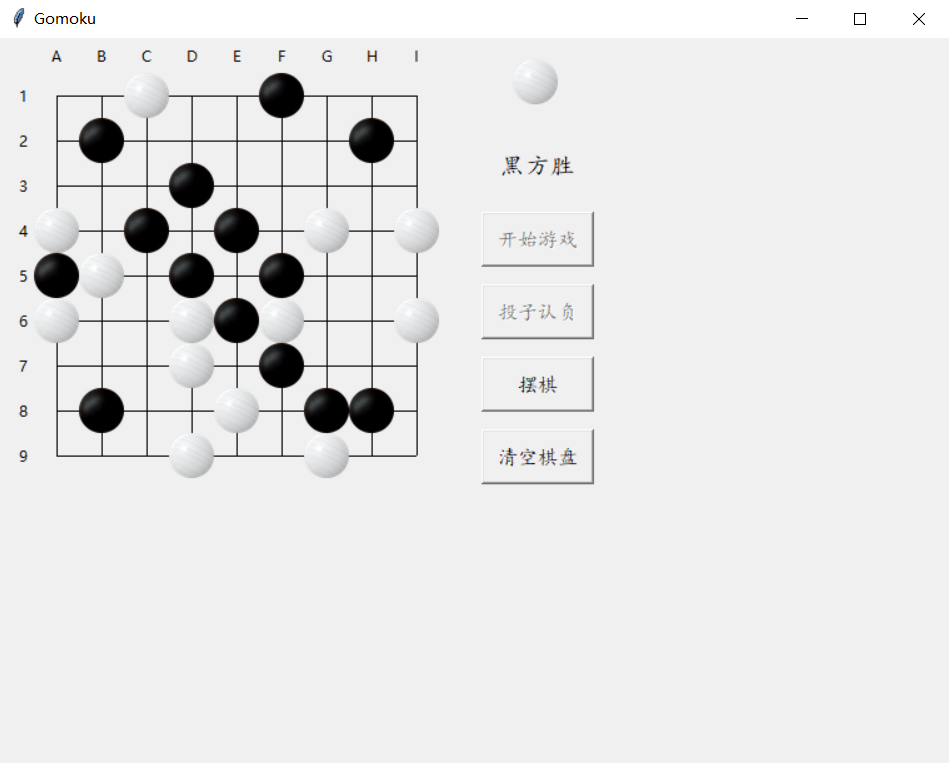
\includegraphics[width=3cm]{uidone.png}
    \end{minipage}
  \end{figure}
\end{frame}

\subsection{蒙特卡洛树搜索}

\begin{frame}{蒙特卡洛树搜索}
  \begin{figure}[htbp]
      \centering
      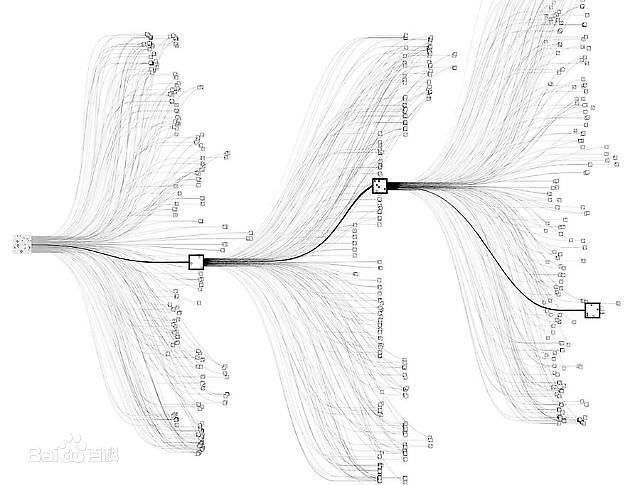
\includegraphics[width=0.6\linewidth]{mc.jpg}
      \caption{MCTS}
  \end{figure}
\end{frame}

\begin{frame}{蒙特卡洛树搜索}
  \begin{block}{AlphaGo-Zero 的 MCTS}
	\begin{itemize}
		\item 由多项式上置信树算法(Polynomial Upper Confidence Tree,PUCT)决定搜索的子节点
		\item 叶节点不使用 Rollout 策略,而是直接使用神经网络进行评估。
	\end{itemize}
  \end{block}
  \begin{figure}[htbp]
	    \centering
	    \begin{minipage}[t]{0.7\textwidth}
	      \centering
	      \includegraphics[width=0.9\linewidth]{puct.png}
	      \caption{PUCT}
	    \end{minipage}
  \end{figure}
\end{frame}

\subsection{神经网络}

\begin{frame}{神经网络}
	\begin{itemize}
		\item 使用 pytorch 模块完成神经网络部分的实现
		\item 网络结构为 pytorch 的 resnet18
	\end{itemize}
	
	\begin{figure}[htbp]
	    \begin{minipage}[t]{0.7\textwidth}
	      \centering
	      
\includegraphics[width=0.9\linewidth]{pytorch.jpeg}
	      \caption{ytorch}
	    \end{minipage}
    \end{figure}
\end{frame}

\section{项目进度}

\begin{frame}{项目进度}
	\begin{block}{项目进度}
		\begin{itemize}
			\setlength{\itemsep}{6pt}
			\item 五子棋对局的前后端开发基本完成
			\item 完成五子棋 AI 的框架书写
			\item 完成初步训练,损失率可以下降
		\end{itemize}
	\end{block}	
	\begin{block}{现阶段问题}
		\begin{itemize}
			\item 损失率达不到预期,实际表现不佳
			\item 猜测模型局限在局部最小值
		\end{itemize}
	\end{block}
\end{frame}

\begin{frame}{解决方案}
	\begin{itemize}
		\item 调整 PUCT 式子中常数 $c_{puct}$ 的大小
		\item 调整迪利克雷噪声浓度
		\item 调整搜索量
		\item 调整数据池大小
		\item 调整 batchsize
		\item 调整初始学习率和学习率变化方式
	\end{itemize}
\end{frame}

\section{预期目标}

\begin{frame}{预期目标}
  \begin{block}{结题}
    \begin{itemize}
      \setlength{\itemsep}{6pt}
      \item 完成五子棋AI
            \begin{itemize}
              \setlength{\itemsep}{6pt}
              \item 较快的运行速度
              \item 较强的对弈水平
              
            \end{itemize}
      \item 完成五子棋对局界面
            \begin{itemize}
	            \setlength{\itemsep}{6pt}
	            \item 支持人机对弈
	            \item 界面简洁友好
	            \item 支持难度调整
            \end{itemize}
            
    \end{itemize}
  \end{block}
\end{frame}

\section{Q\&A}

\begin{frame}{\secname~ }
  \begin{center}
    \huge{That's all. Thank you!}\\
    \vspace{1cm}
    \huge{Q\&A}
  \end{center}
\end{frame}

\end{document}
